\documentclass[preprint,12pt,times,a4paper]{elsarticle}

\usepackage{graphicx}
\usepackage{amssymb}
\usepackage{amsmath}
\usepackage{lineno}
\usepackage{xspace}
\usepackage{lipsum}
\usepackage{cleveref}
\usepackage{stackengine}
\usepackage{titlesec}
\usepackage{xcolor}
\usepackage[bitstream-charter]{mathdesign}
\usepackage[T1]{fontenc}
\usepackage{geometry, float}
\usepackage{biblatex}
\addbibresource{paper.bib}

\geometry{a4paper}

\usepackage[normalem]{ulem}
\usepackage{stackengine}

\journal{Nuclear Instruments and Methods in Physics Research A}

\newcommand{\XGB}{XGBoost}

\begin{document}

\begin{frontmatter}

\setcounter{page}{0}
\title{Simulation Study of Angular Resolution of a New Electromagnetic Sampling Calorimeter}

\author[jbnu]{Junlee~Kim}
\ead{junlee.kim@cern.ch}
%\cortext[cor1]{Corresponding author. Tel.: +82-xxxxxxxxx.}

\author[jbnu]{Eun-Joo~Kim\corref{cor1}}
\ead{ejkim@jbnu.ac.kr}
\cortext[cor1]{Corresponding author. Tel.: +82-10-4581-5649.}

\author[korea]{Young~Jun~Kim}
\author[korea]{Jung~Keun~Ahn}
\author[kek]{Gei~Youb~Lim}

\address[jbnu]{Division of Science Education, Jeonbuk National University, Jeonju 54896, Korea}
\address[korea]{Department of Physics, Korea University, Seoul 02841, Korea}
\address[kek]{Institute of Particle and Nuclear Studies (IPNS), High Energy Accelerator Research Organization (KEK), Tsukuba 305-0801, Japan}

%\date[]{Received 6 August 2007}

\begin{abstract}
We report simulation results on the angular resolution of electromagnetic (EM) sampling calorimeters with photons being in the range of 100~MeV to 2~GeV. A simulation model of the EM calorimeter consists of alternating layers of a 1-mm-thick Pb plate and a 5-mm-thick plastic scintillator plate. The scintillator plates are alternatively segmented in horizontal and vertical strips. In this study, we obtained energy deposits in individual strips using Geant4 simulations and reconstructed incident photon angles using a XGBoost model with boosted decision trees. Angular resolutions are studied in terms of the strip width.
The 15-mm-wide strips provide acceptable angular resolution of 1.23~$\pm$~0.01$^{\circ}$. Incident photon directions can be well reconstructed in the front part (6.2$X_{0}$) of the EM calorimeter with the acceptable angular resolution of 
1.30~$\pm$~0.01$^{\circ}$. The angular resolution varies significantly with the incident photon energy, and weakly dependent on the incidence angle. The energy dependence can be expressed as $\sigma_{\theta}= p_{0} \oplus p_{1} /\sqrt{E_{\gamma}}$. For low energy photons, the angular resolution is dependent on the incidence angle, and the dependence disappears as the incident energy increases. For the $\theta>$~10 deg, $p_{0}$ and $p_{1}$ are estimated to be 0.29$^{\circ}$ and 1.24$^{\circ}$, respectively.

\end{abstract}
\begin{keyword}
% keywords here, in the form: keyword \sep keyword
Electromagnetic Calorimeter \sep Geant4 \sep XGBoost \sep KOTO
\end{keyword}

\end{frontmatter}

\section{Motivation}
\label{sec:mot}
Electromagnetic (EM) calorimeter plays an important role in experimental studies for the nuclear and particle physics. Various materials have been developed for better energy and timing resolutions so far~\cite{Calorimeter}. EM calorimeters can be divided into two groups: sampling calorimeters and homogeneous calorimeters. Sampling calorimeters consist of alternating layers of an absorber generating EM showers and an active medium providing signals. On the other hand, homogeneous calorimeters are built of only a single type of material that facilitates both EM showers and signal generations. Today, the sampling calorimeter becomes very popular in large-scale high energy experiments, owing to its cost-effectiveness. In sampling calorimeters the energy deposited in the active medium fluctuates because the active layers are interleaved with absorber layers. This so-called sampling fluctuation dominates the energy resolution.

The sampling fluctuation can be improved by optimizing the thickness ratio of the absorber to the active medium. A 3-m-long cylindrical calorimeter made of alternating layers of Pb and plastic scintillator plates is an example of the sampling calorimeter~\cite{Murayama:2020mcp}.

The segmented structure of the active medium facilitates the measurement of lateral distributions of the EM shower along the incident photon direction. The photon direction can also be deduced from the information on the EM shower shape. The measurement of photon directions can help predict photon production vertices, which is crucial for the background suppression in KOTO experiment~\cite{KOTO:2012}.

Stochastic behaviors of the EM shower development limit to the angular resolution of the photon direction measurement. Energy deposits in each active layer of a sampling calorimeter fluctuate event by event so that the reconstruction of photon directions necessitates the longitudinal and lateral segmentation of the calorimeter.

This paper describes a machine learning approach based on XGBoost (XGB) model~\cite{xgboost:2016} with boosted decision trees in order to reconstruct the direction of incident photons entering a sampling calorimeter with alternating layers of a Pb plate and plastic scintillator strips in horizontal and vertical directions. We generated EM showers in a sampling calorimeter using Geant4 simulations. We report on the detector configuration providing the acceptable angular resolution, and report on the angular resolution of the EM sampling calorimeter in terms of the incidence angle and the incident energy.

\section{Electromagnetic Shower Simulation}
\label{sec:ems}

\begin{figure}[!hbt]
\centering
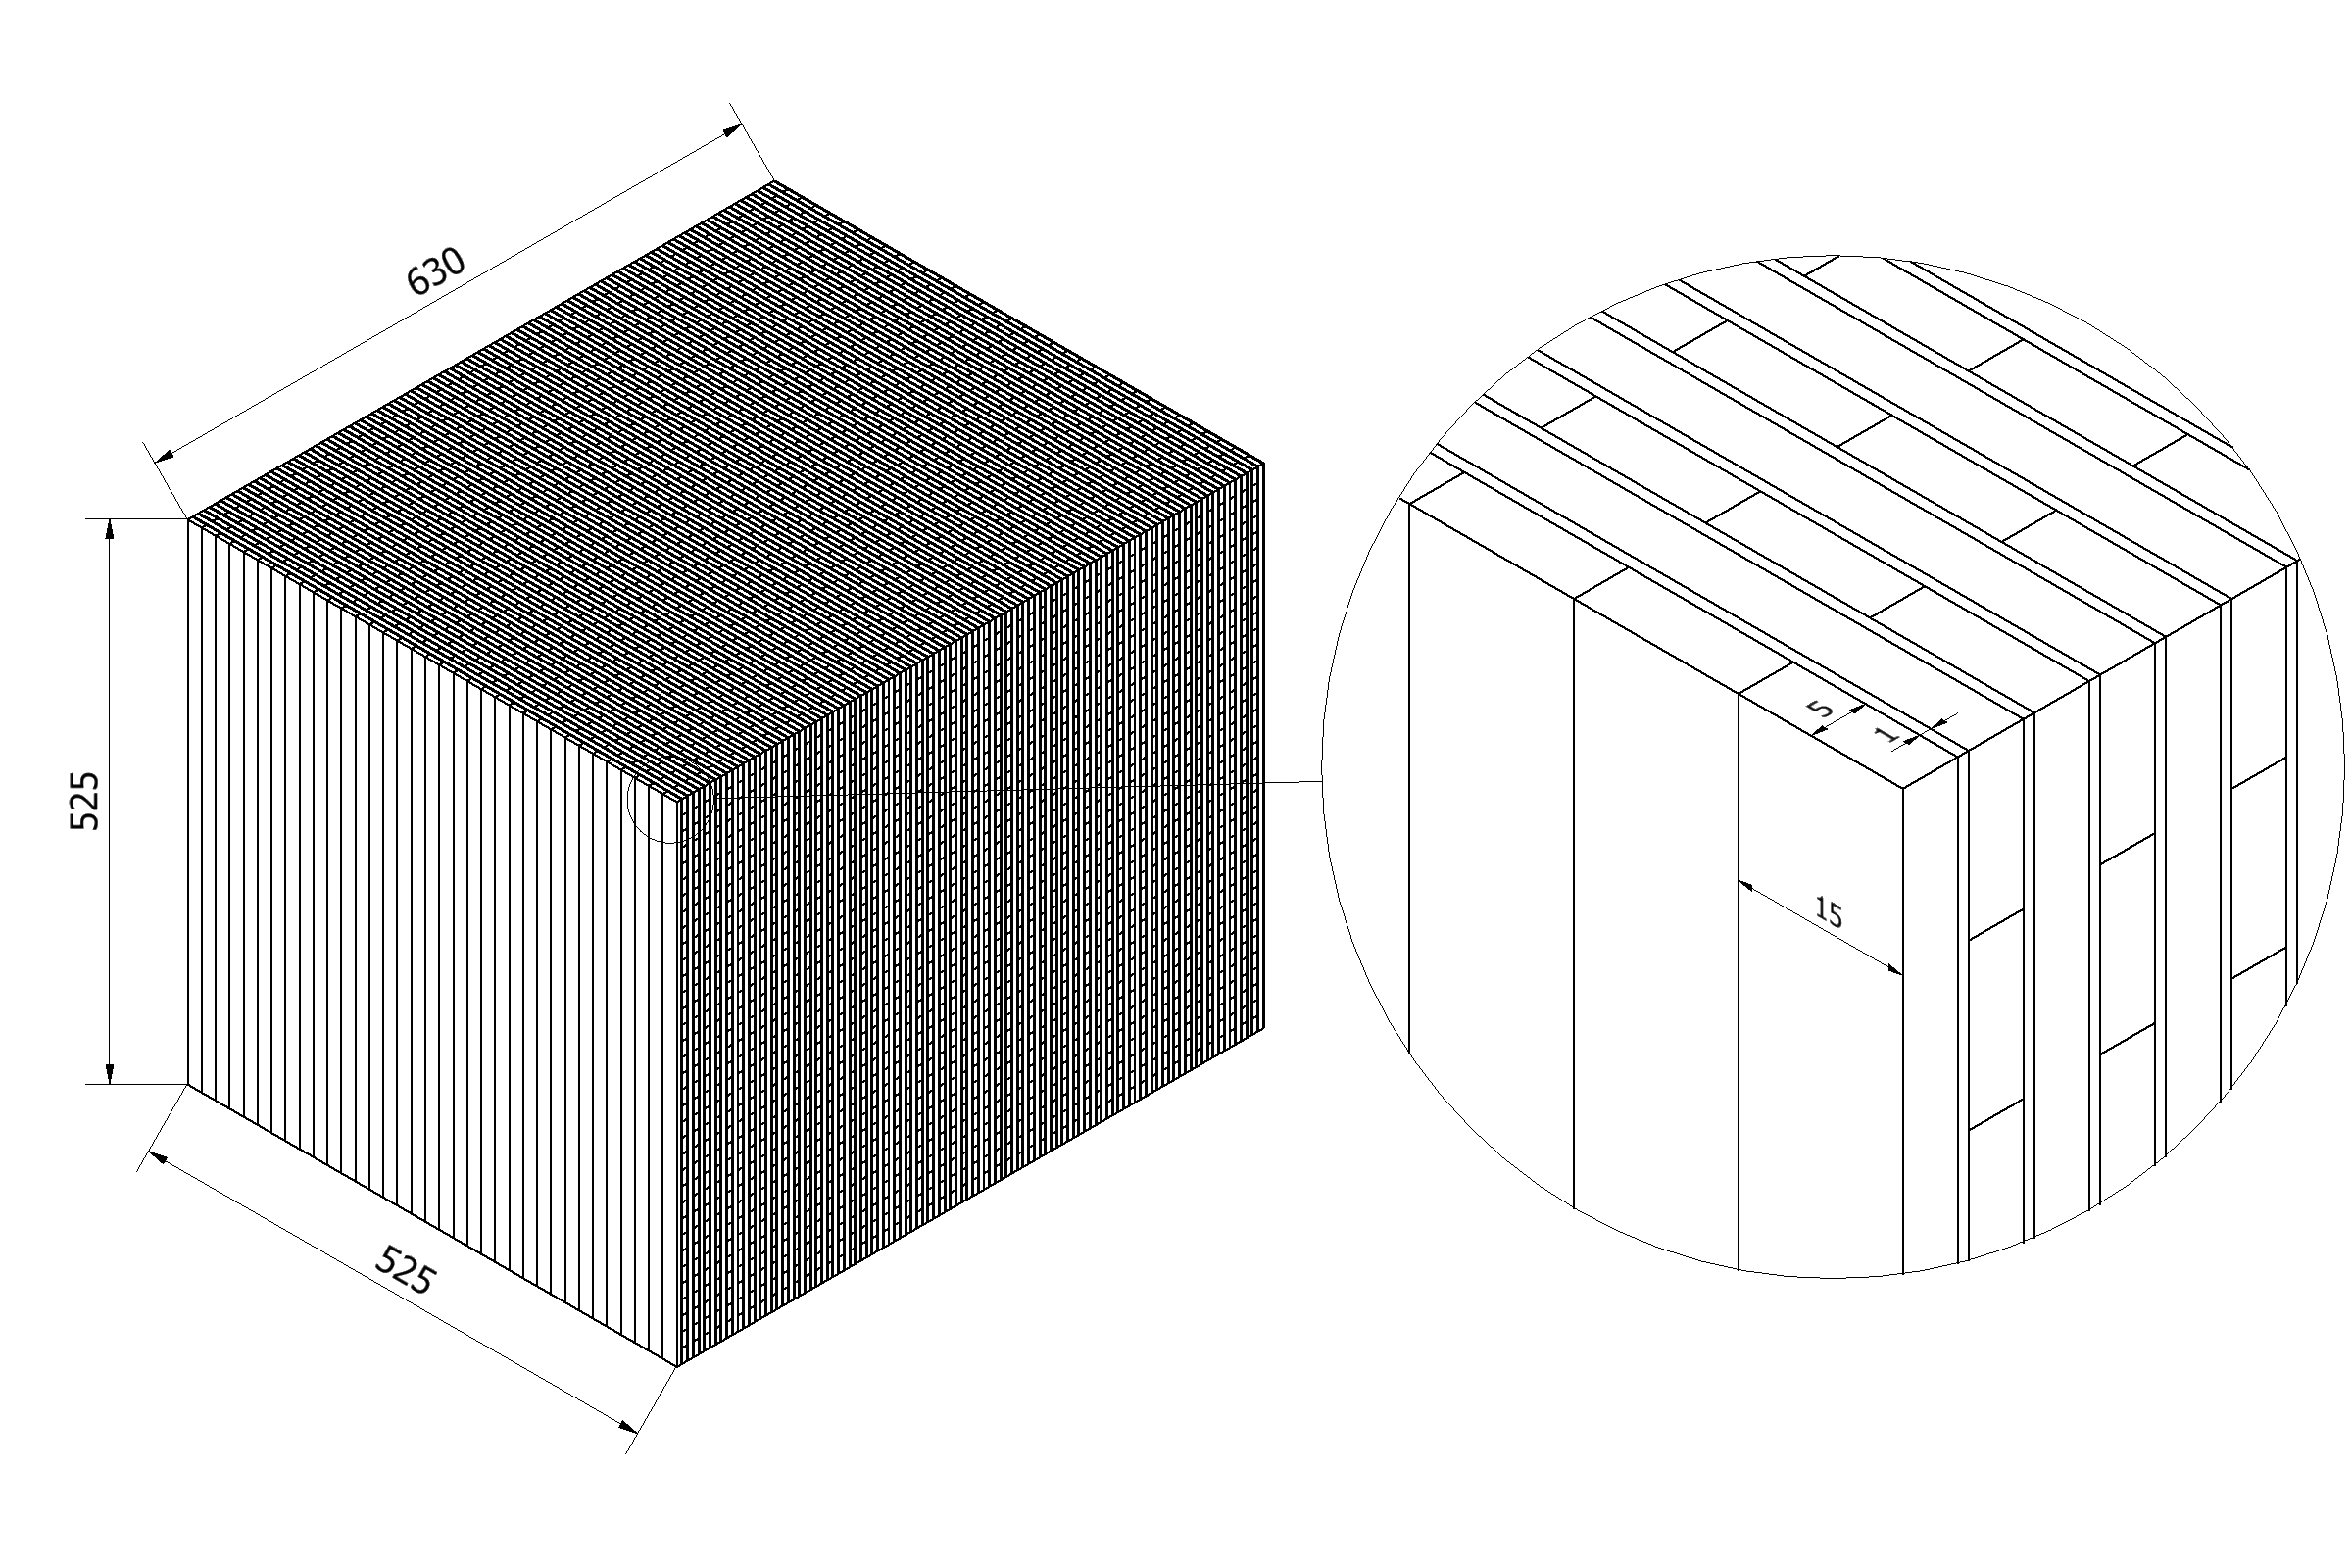
\includegraphics[width=0.6\textwidth]{figures/Fig1_detector_schematic.jpeg}
\caption{ Schematic of the sampling calorimeter model consisting of 105 alternating layers of a Pb plate and a segmented scintillator plate in 35 strips. Each scintillator plate is oriented alternatively in horizontal and vertical directions. See text for details. }
\label{fig:det_conf}
\end{figure}

Simulation models of a sampling calorimeter were constructed as a block consisting of alternating layers of a 1-mm-thick Pb absorber and a 5-mm-thick polyvinyltoluene-based plastic scintillator. The plastic scintillator is segmented in 15-mm-wide strips, which are alternatively oriented in vertical and horizontal directions as shown in Fig.~\ref{fig:det_conf}. The sampling calorimeter model has a cross-section of 525~$\times$~525~mm$^{2}$ and accommodates 105 alternating layers of 630~mm length (20$X_{0}$), which is sufficiently long to absorb full photon energy in the range of 100~MeV to 2~GeV. 

\begin{figure}[!hbt]
\centering
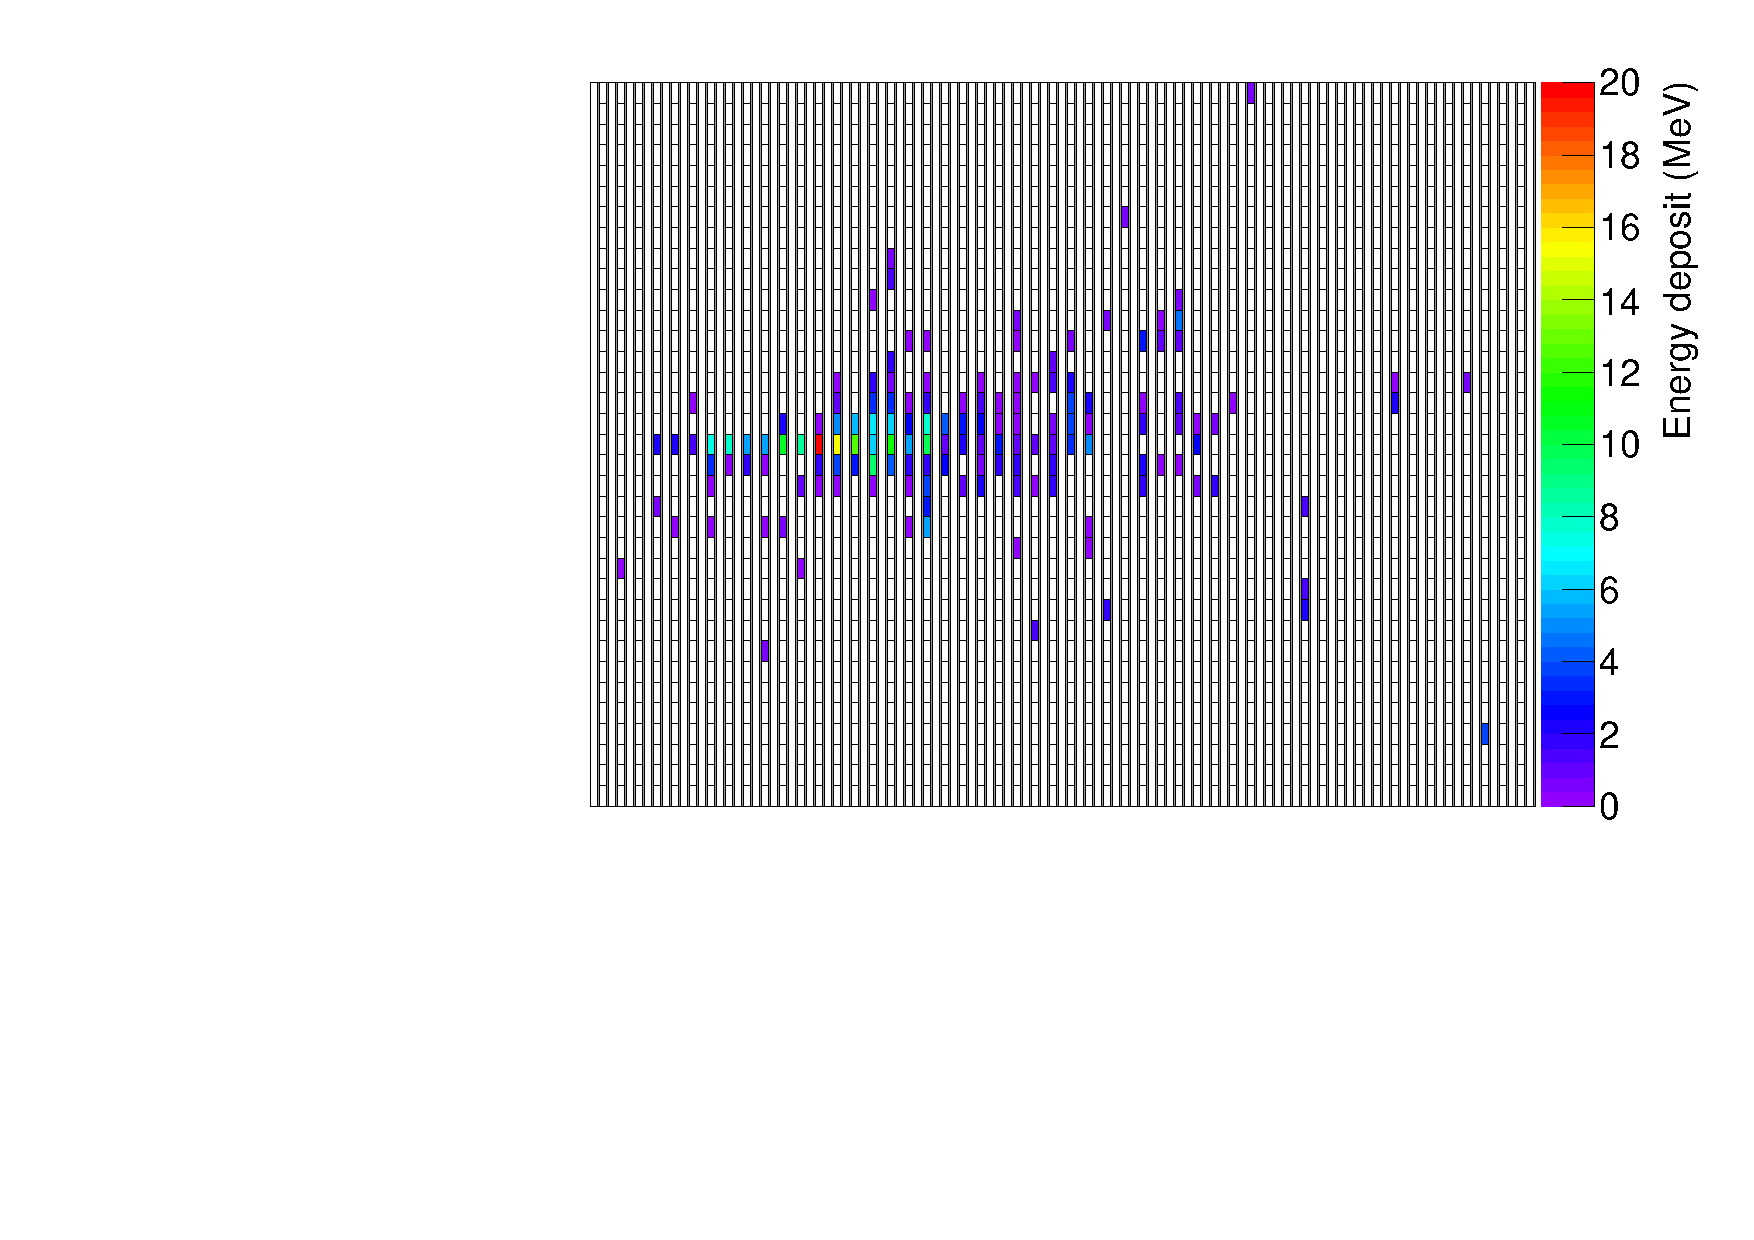
\includegraphics[width=0.48\textwidth]{figures/Fig2_EMShower_XZ.pdf}
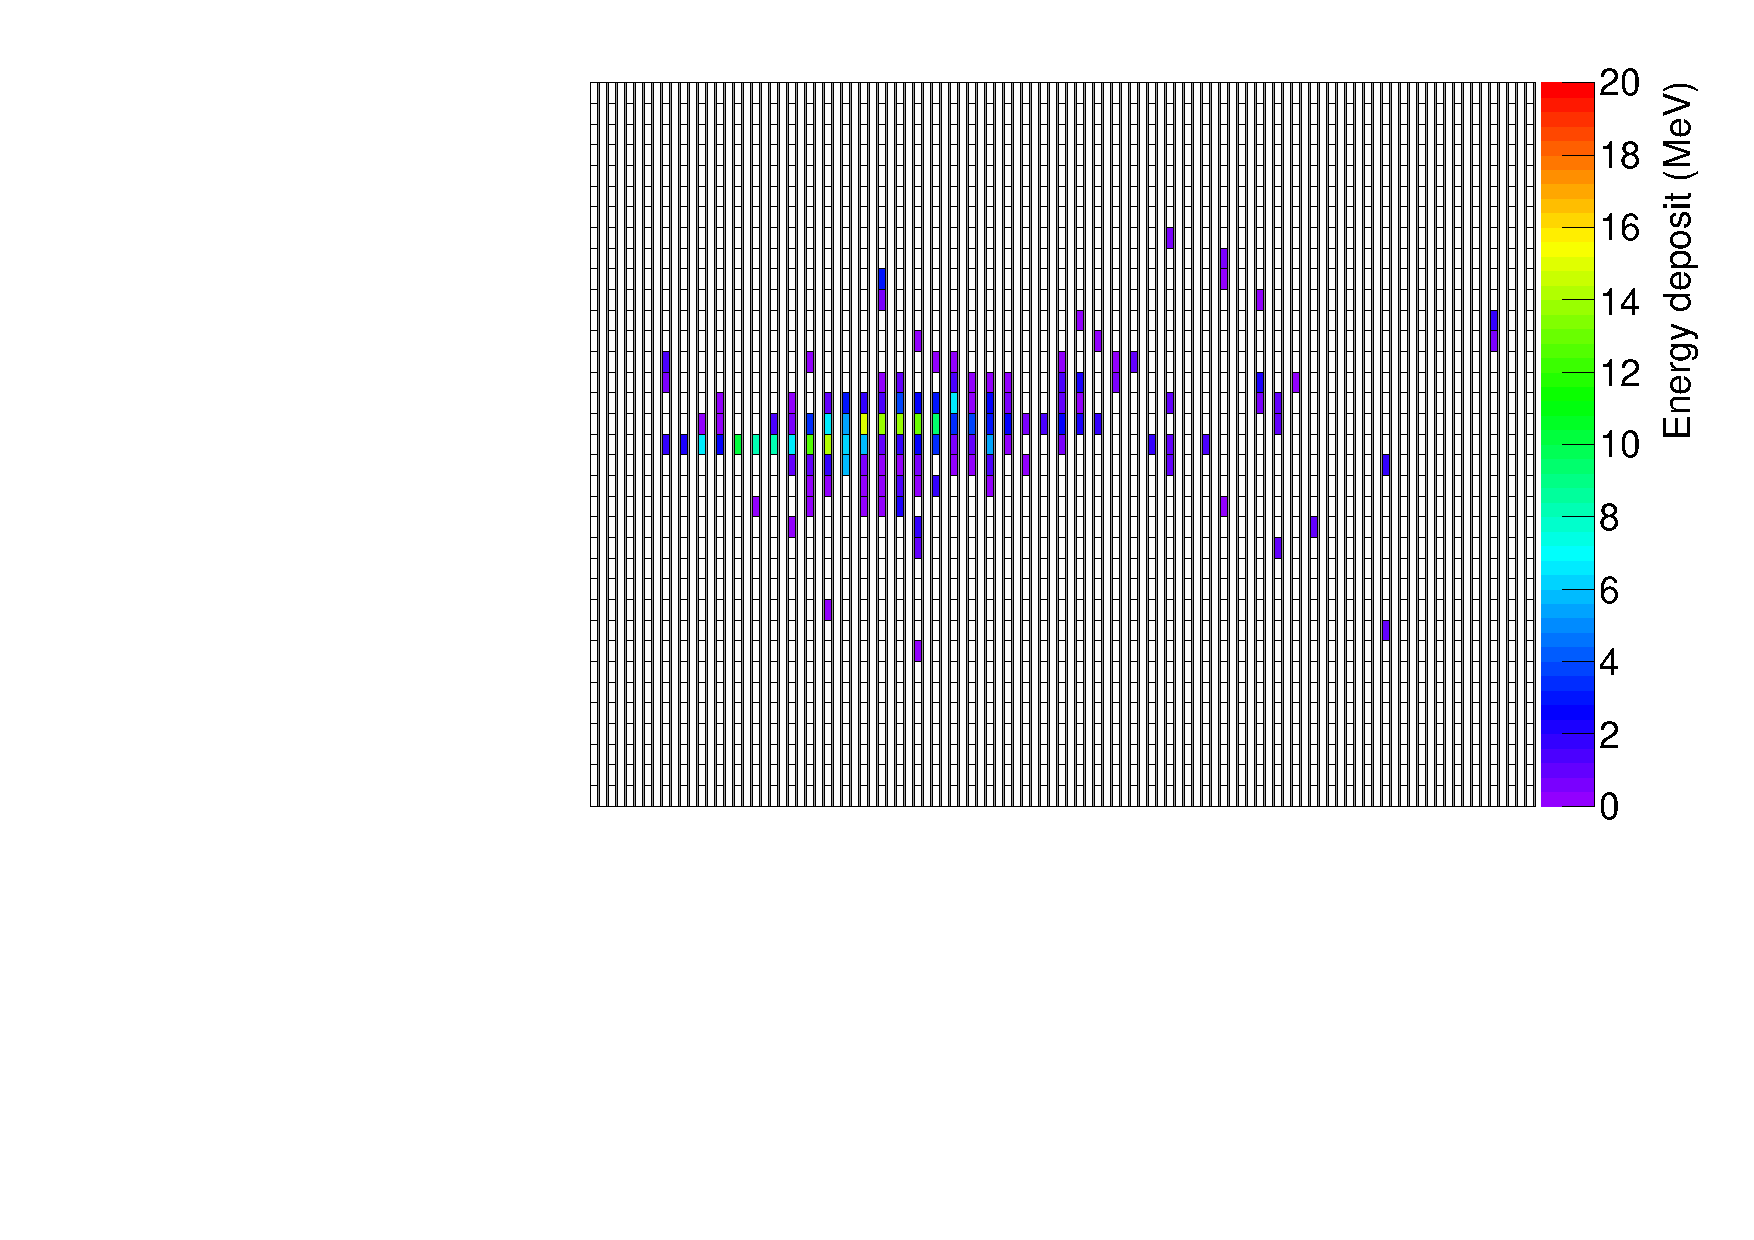
\includegraphics[width=0.48\textwidth]{figures/Fig2_EMShower_YZ.pdf}
\caption{ Event display of simulated energy deposit patterns for a 1-GeV photon entering the calorimeter ($\theta=$~0) in (a) $xz$- and (b) $yz$-planes.}
\label{fig:Evt_Dis}
\end{figure}

The detector response to incident photons was simulated using Geant4 (ver. 4.10.06) with the standard EM sub-packages~\cite{GEANT4}. The beam direction defines the $z$-axis. The photon direction is defined as polar angle ($\theta$) with respect to the $z$-axis. Figure~\ref{fig:Evt_Dis} illustrates simulated energy deposit patterns in each strip for a 1-GeV photon at a normal incidence in $xz$- and $yz$-planes. Each segmented region in Fig.~\ref{fig:Evt_Dis} represents each channel.

\section{Reconstruction of Incidence Angles}
\label{sec:res}

Incidence angles of photons are reconstructed using the XGB model that is a scalable machine learning system for the gradient boosting tree~\cite{xgboost:2016}. A machine learning model maps a set of data inputs, known as features, to target variables. In this study, the XGB model maps a dataset of energy deposits in each scintillator strip to an incidence angle of a photon. Training data were carefully prepared using Geant4 simulation such that the input datasets are representative of a detector response of real sampling calorimeters. To minimize data bias, the incidence angles were uniformly generated at the detector surface in the angular range of 0~$<\theta<$~50$^{\circ}$ and 0~$<\varphi<$~360$^{\circ}$, where $\varphi$ denotes azimuthal angle. Such a wide angular coverage provides good training datasets for the XGB. The number of training samples is $10^{5}$ considering limited computing resources. To test the reconstruction of incidence angles, we generated photons at a fixed incidence angle $\theta$. Note that the incident energy is known.

\begin{figure}[!hbt]
\centering
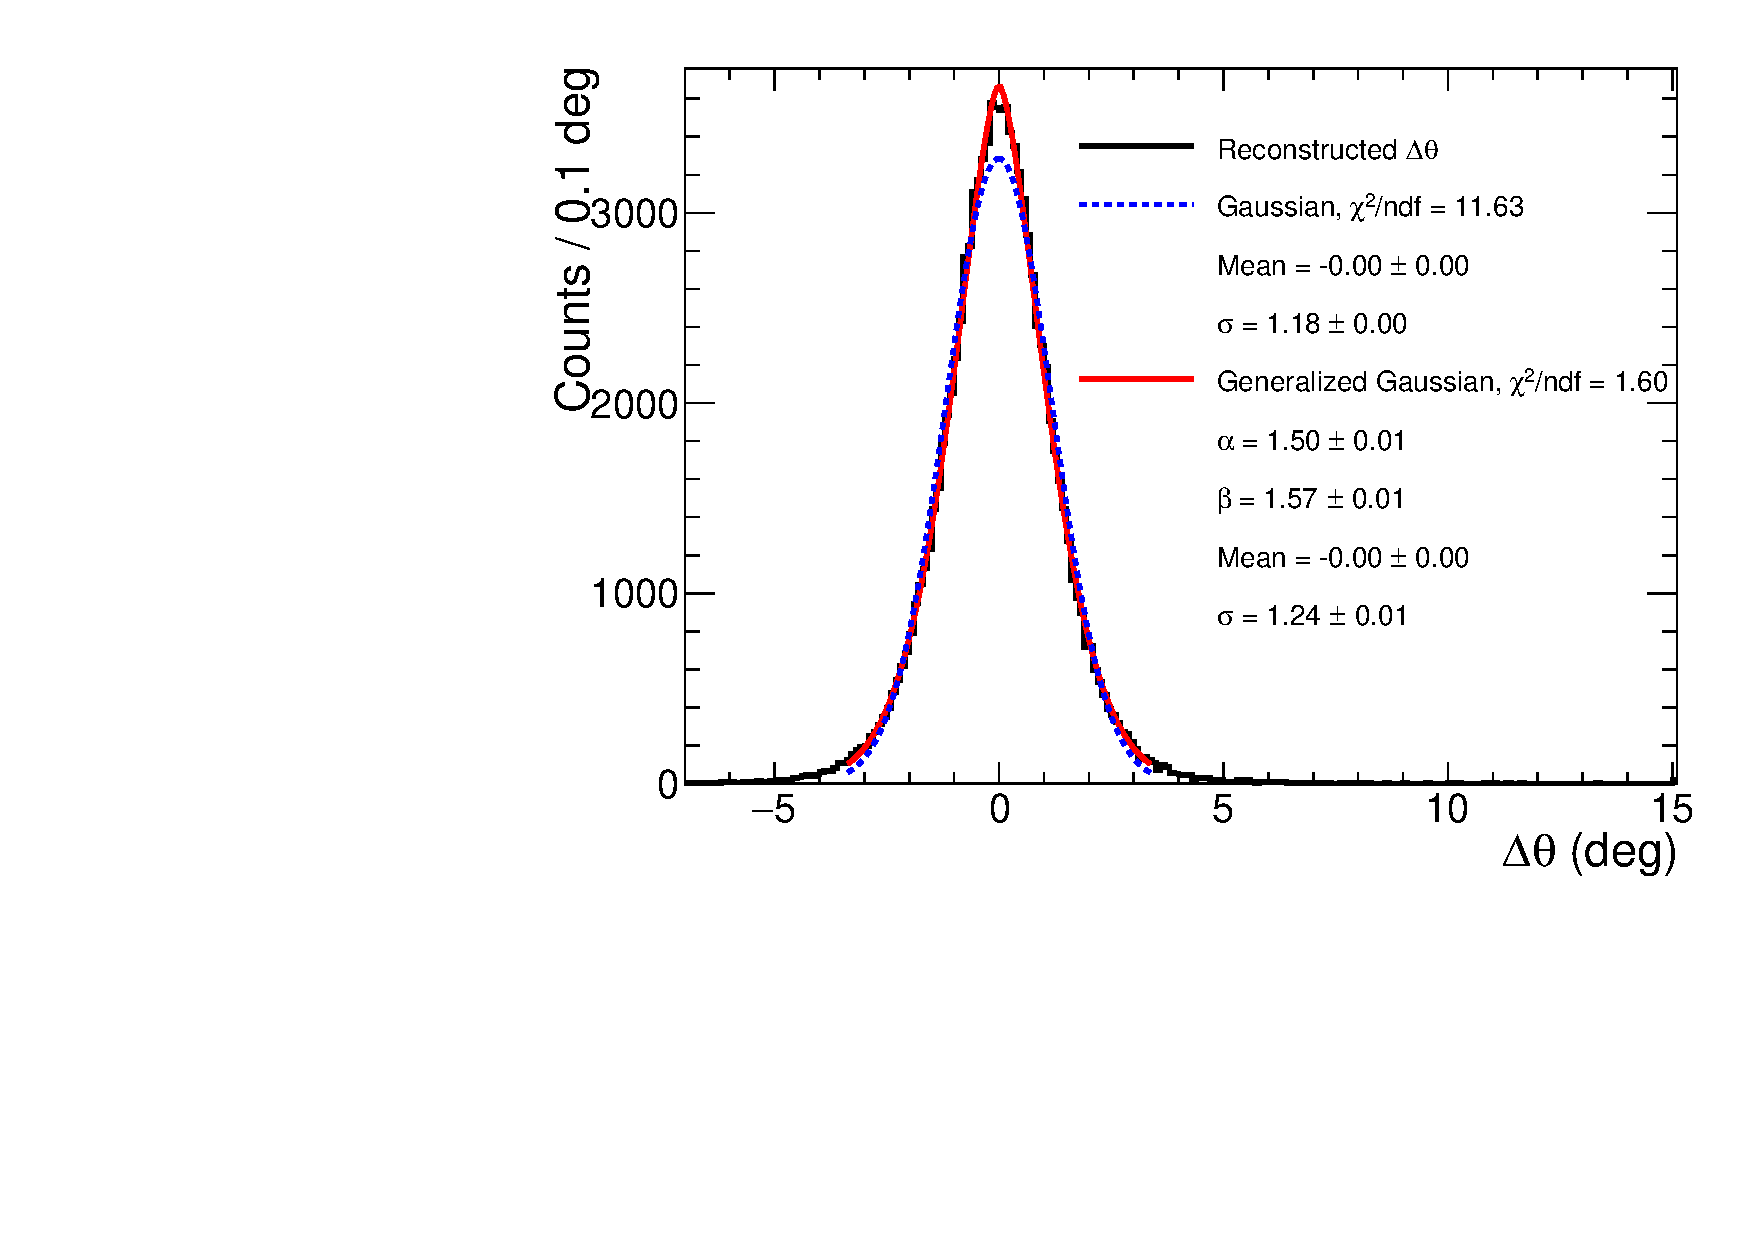
\includegraphics[width=0.7\textwidth]{figures/Fig3_fit_GG.pdf}
\caption{ The relative incidence angle for 1-GeV photons generated at $\theta=$~10$^{\circ}$. The distribution is fitted with the Gaussian and the Generalized Gaussian function. The later gives a better result.}
\label{fig:angle_10degree}
\end{figure}

Figure~\ref{fig:angle_10degree} represents a distribution of the relative incidence angle ($\Delta\theta$) for 1-GeV photons generated at $\theta=$~10$^{\circ}$. $\Delta\theta$ represents the radial displacement of the reconstructed incidence angle from the true incidence direction. The central 98\% part of the distribution is fitted with the Gaussian function and the Generalized Gaussian (GG) function. We tested two functions, Gaussian and GG to describe the reconstructed angle distribution. The GG function, also known as the generalized error distribution, is expressed as
\begin{eqnarray} 
f(x; \mu, \alpha, \beta) = \frac{\beta}{2 \alpha \Gamma(1/\beta)}e^{-(|x-\mu|/\alpha)^\beta},
\label{eqn:gg}
\end{eqnarray}
where $\mu$ denotes a mean value. Parameters $\alpha$ and $\beta$ determine the scale and shape of the distribution, respectively. Variance of the GG function is given by $\sigma^2 \equiv \alpha^2 \Gamma(3/\beta) / \Gamma(1/\beta)$. The angular resolution of the incidence angle reconstruction is defined as $\sigma$.

\begin{figure}[!hbt]
\centering
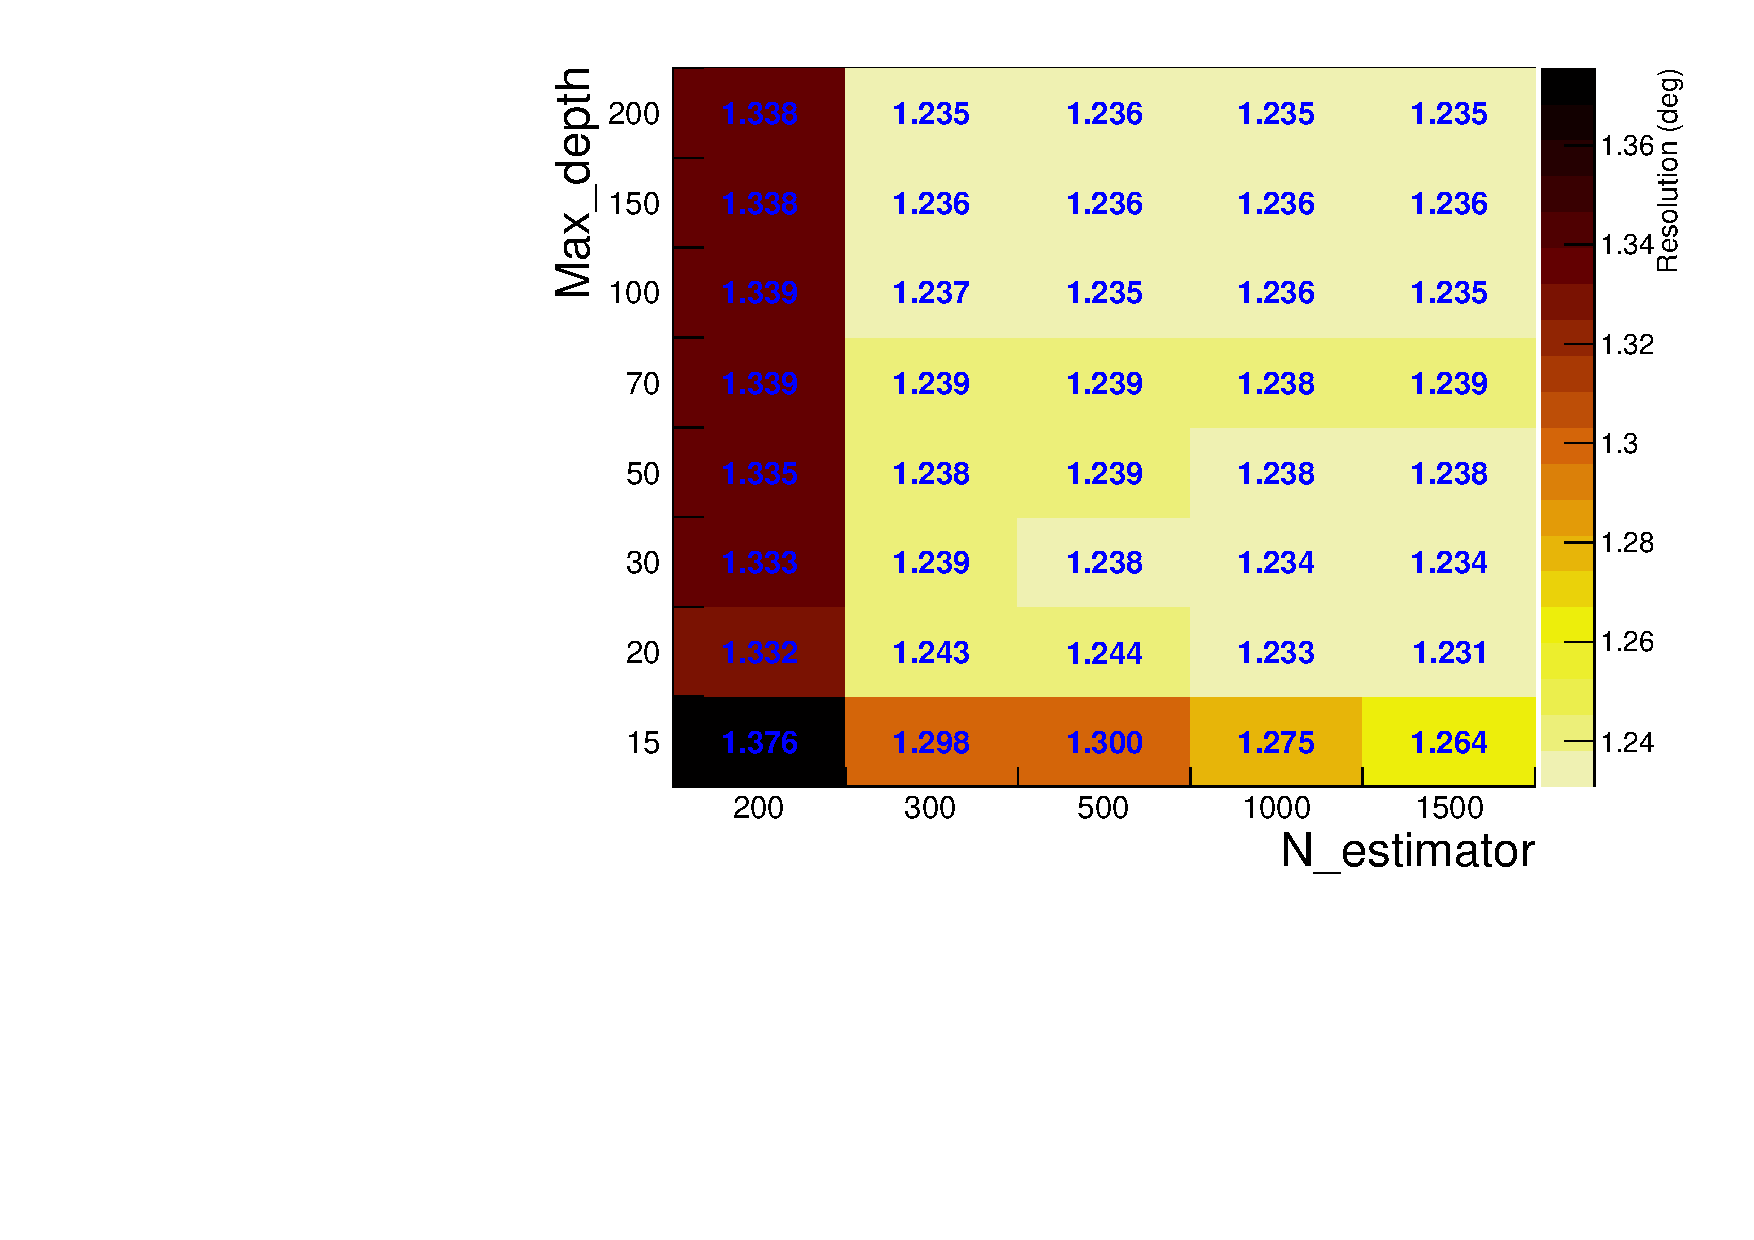
\includegraphics[width=0.69\textwidth]{figures/Fig4_Opt.pdf}
\caption{Angular resolutions are displayed in terms of combination of N\_estimators and Max. depth. The best angular resolution is obtained with N\_estimators~=~300 and Max. depth~=~100. }
\label{fig:par_scan}
\end{figure}

We studied a correlation between byperparameters of the XGB model and the angular resolution. The test scans the evaluated angular resolution with different hyperparameters. Figure~\ref{fig:par_scan} shows the test results with N\_estimators and Max. depth. N\_estimators defines the maximum allowed number of decision trees to be developed, and the Max. depth defines the complexity of the structure of decision trees. The best hyperparameter combination was searched for in terms of the angular resolution. As a results, N\_estimators and Max. depth are set to 300 and 100, respectively. Similar tests were also performed for different hyperparameters. The best values for other hyperparameters are displayed in Tab.~\ref{tab:XgbPar}. Other hyperparameters tuned in this study are Subsample, Learning rate, and Gamma. Subsample controls the fraction of total event samples for each boosting procedure, and Learning rate weights a decision tree to be added onto the current model. Lastly, Gamma regulates the evaluation of each decision tree. It is also worth mentioning that the fraction of the tail is not changing from 2\%.
\begin{table}[hbt!]{\small
\centering
\caption{Hyperparameters of the XGB model}
\begin{tabular}{cccc}
\hline 
Parameter & Function & Default value & Used value \\ \hline 
N\_estimators & The number of decision trees & N.A. & 300 \\  
Max. depth & Possible maximum depth of tree structure & 6 & 100 \\ 
Subsample & Fraction of total data used for a single decision & 1 & 0.8 \\ 
Learning rate & Step length for calculation & 0.3 & 0.02 \\ 
Gamma & Requirement on minimum loss function & 0 & 0 \\ 
\hline
\end{tabular}
\label{tab:XgbPar}
}\end{table}

\begin{figure}[!hbt]
\centering
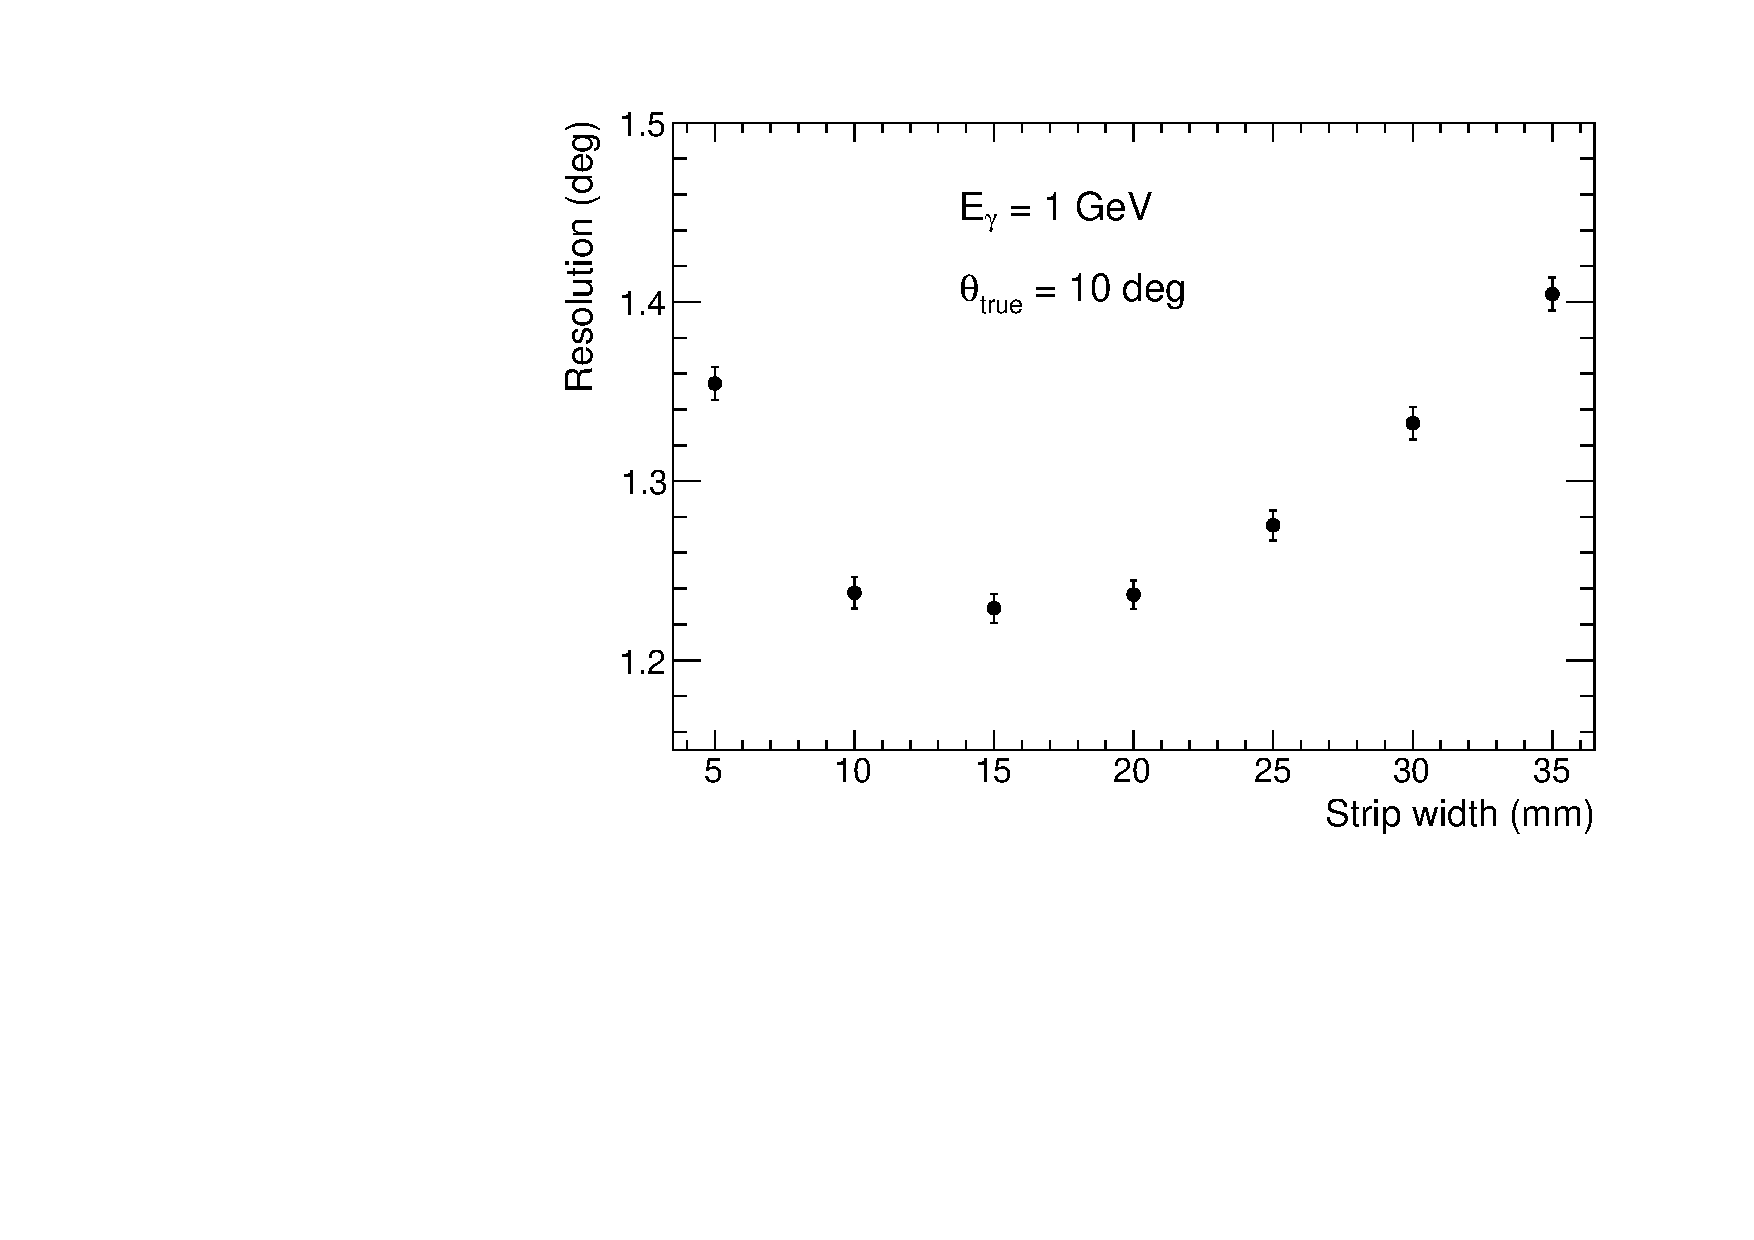
\includegraphics[width=0.58\textwidth]{figures/Fig5_width.pdf}
\caption{ Angular resolutions are deduced in terms of the strip width for 1-GeV photons at $\theta=$~10$^{\circ}$ }
\label{fig:angle_reco_width}
\end{figure}

Angular resolutions were deduced with varying strip widths from 5 mm to 35 mm as shown in Fig.~\ref{fig:angle_reco_width}. The 15-mm-wide strips yield good angular resolution of 1.23~$\pm$~0.01$^{\circ}$. The shorter the strip width is, the larger size of features, which can influence negatively in machine learning. For longer strips, the EM shower information can hardly be obtained.

\begin{figure}[!hbt]
\centering
\stackinset{c}{0.cm}{b}{-0.4cm}{(a)}{
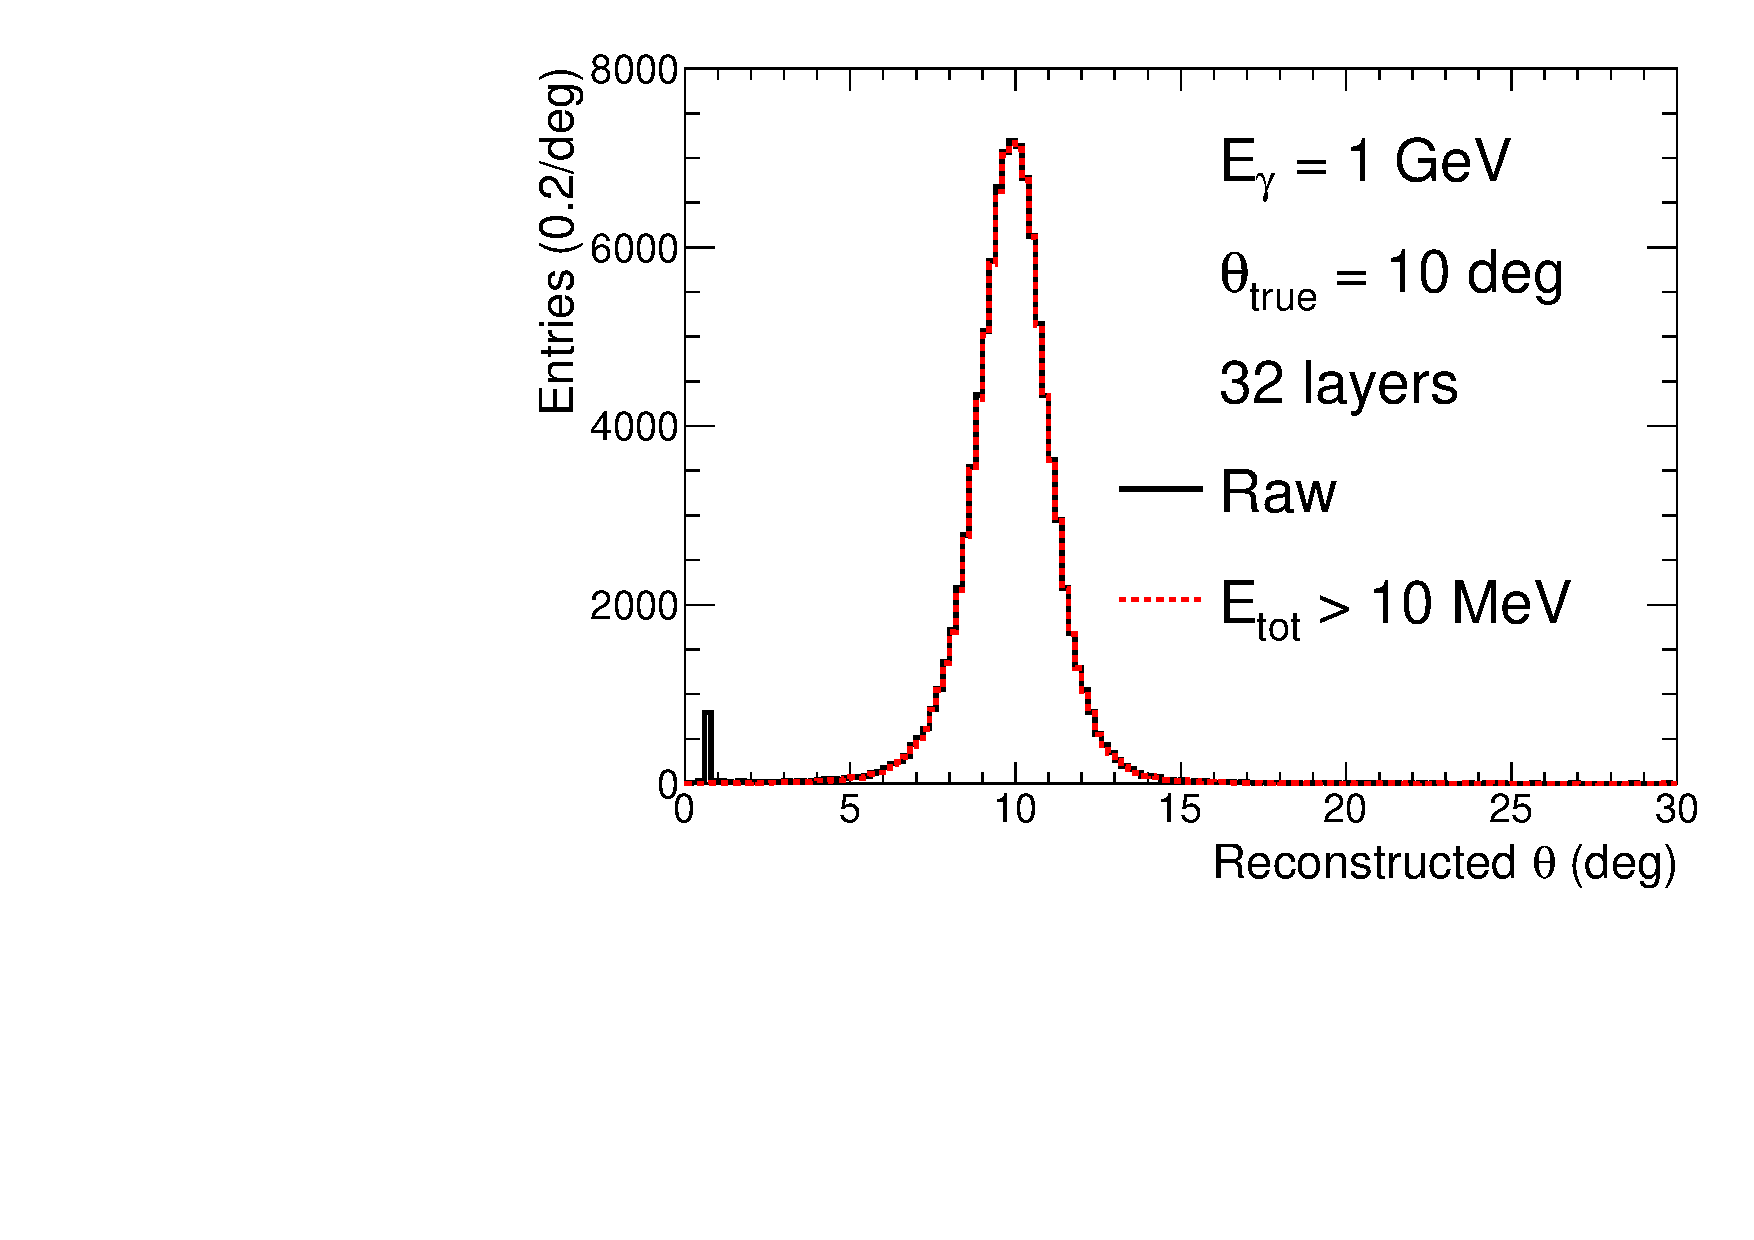
\includegraphics[width=0.48\textwidth]{figures/Fig6_layer_comp.pdf}
}\stackinset{c}{0.cm}{b}{-0.4cm}{(b)}{ 
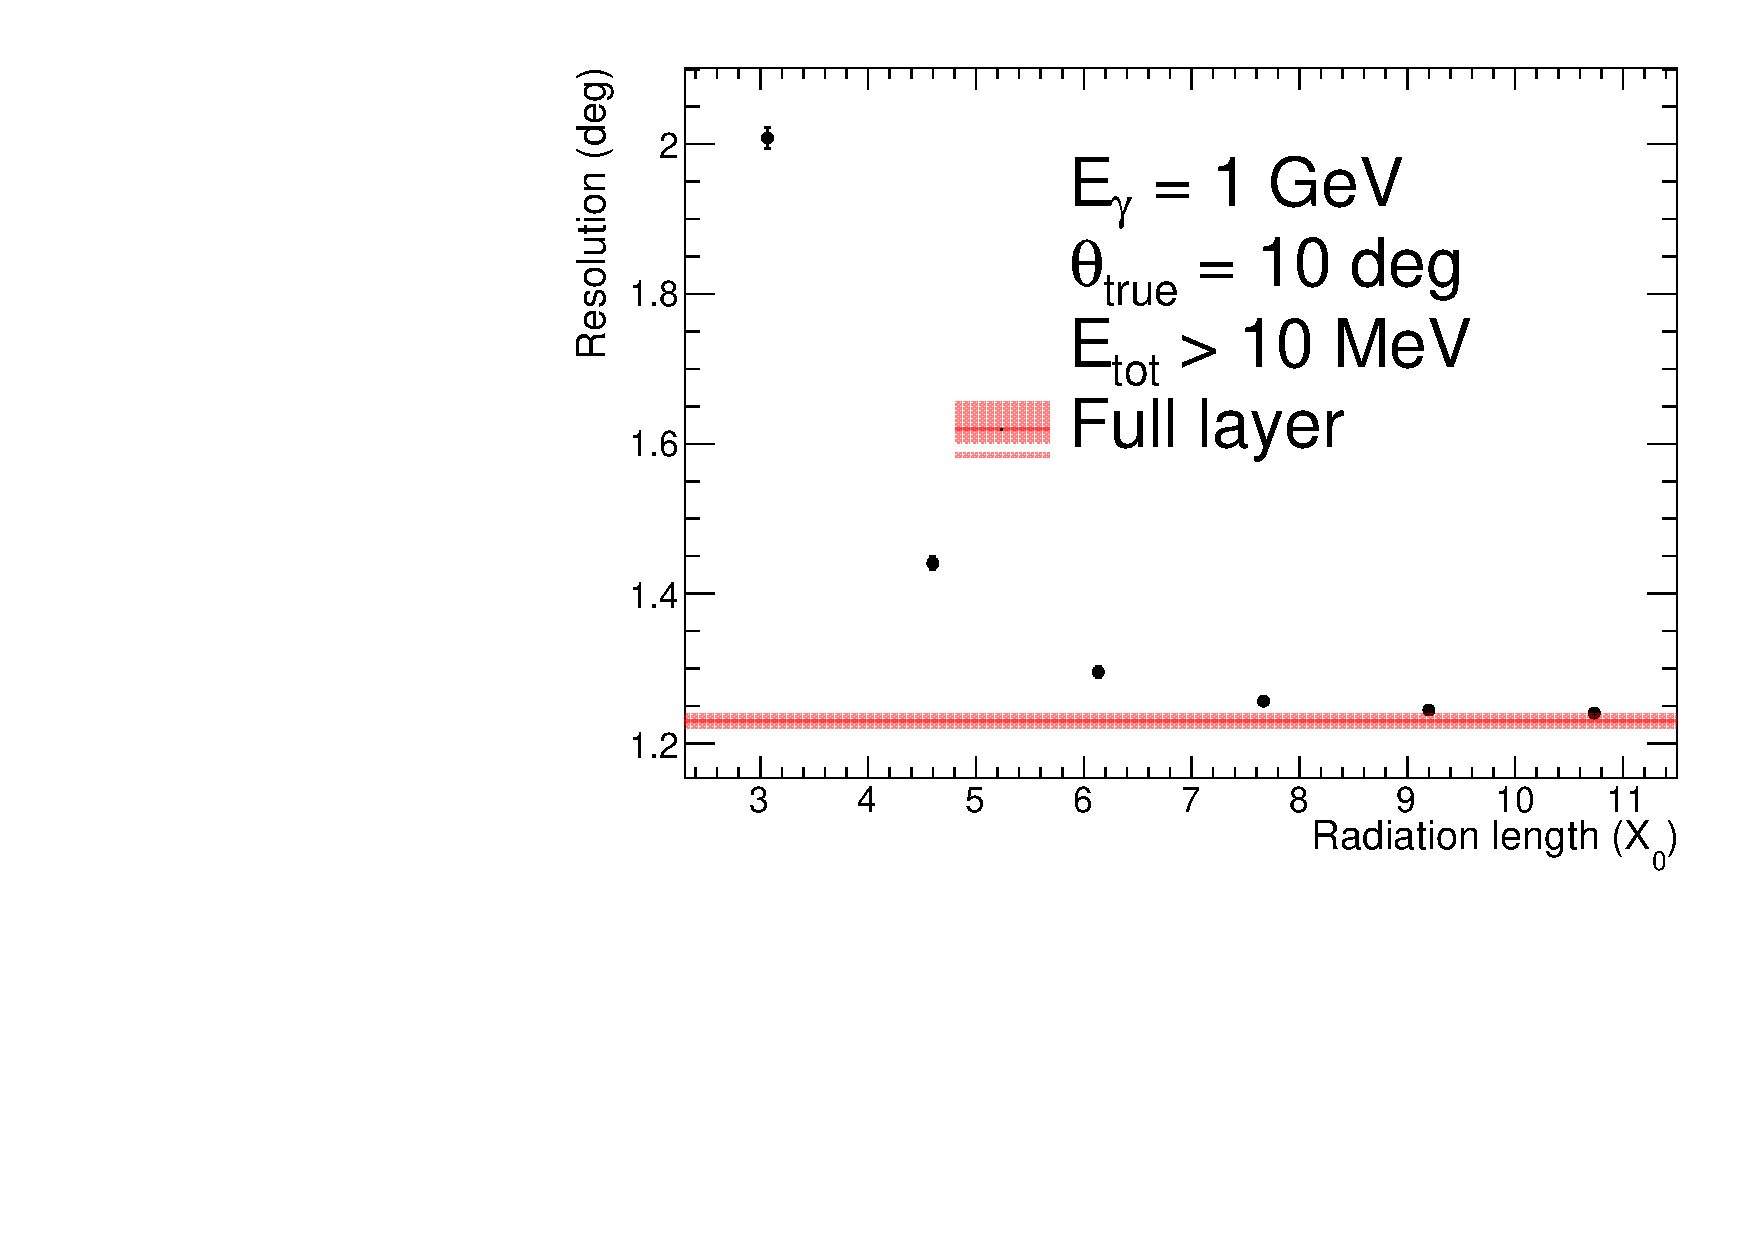
\includegraphics[width=0.48\textwidth]{figures/Fig6_nlayer.pdf}
}
\caption{ (a) Reconstructed polar angles ($\theta$) for 1-GeV photons at $\theta=$~10$^{\circ}$. Red histogram represents the polar angle distribution by requiring $E_{\rm{tot}}>$~10~MeV. (b) Angular resolution as a function of radiation length ($X_{0}$).}
\label{fig:angle_reco_layer}
\end{figure}

Furthermore, incidence angles are reconstructed with the front layers of 6.2$X_{0}$ in which more than 99\% of incident photons generate EM showers. Figure~\ref{fig:angle_reco_layer} (a) shows reconstructed angles using front 32 layers of the detector, which correspond to 6.2$X_{0}$ for 1-GeV photons. A fraction of photons failed to be reconstructed due to the lack of active layers. The failed events are represented as a delta function near 0, and such events are removed by requiring the total energy deposit to be larger than 10~MeV, 1\% of the incident energy. The angular resolution with the front layer is estimated to be 1.30~$\pm$~0.01$^{\circ}$ while possessing inefficiency estimated to be 1.9\%.

\begin{figure}[!hbt]
\centering
\stackinset{c}{0.cm}{b}{-0.4cm}{(a)}{
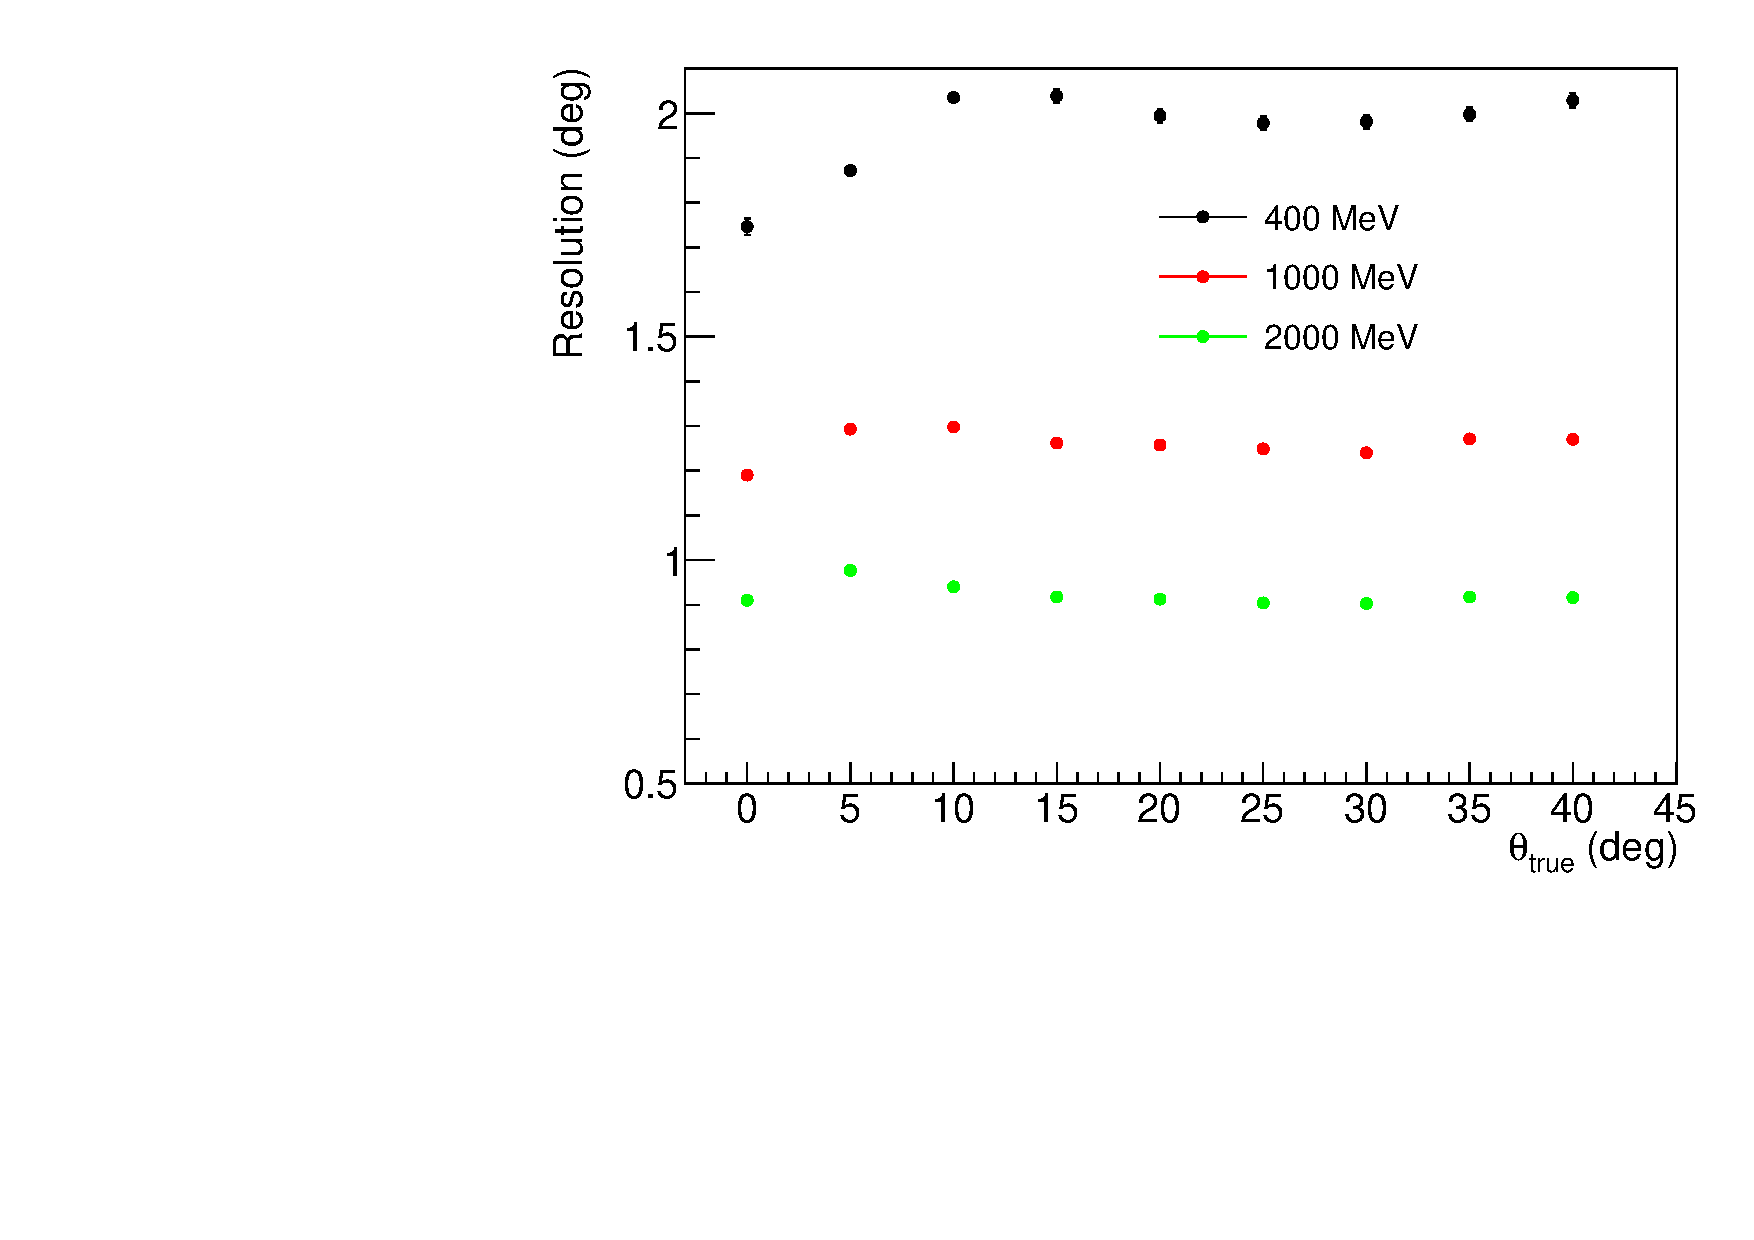
\includegraphics[width=0.44\textwidth]{figures/Fig7_res_ene.pdf}
}\stackinset{c}{0.cm}{b}{-0.4cm}{(b)}{
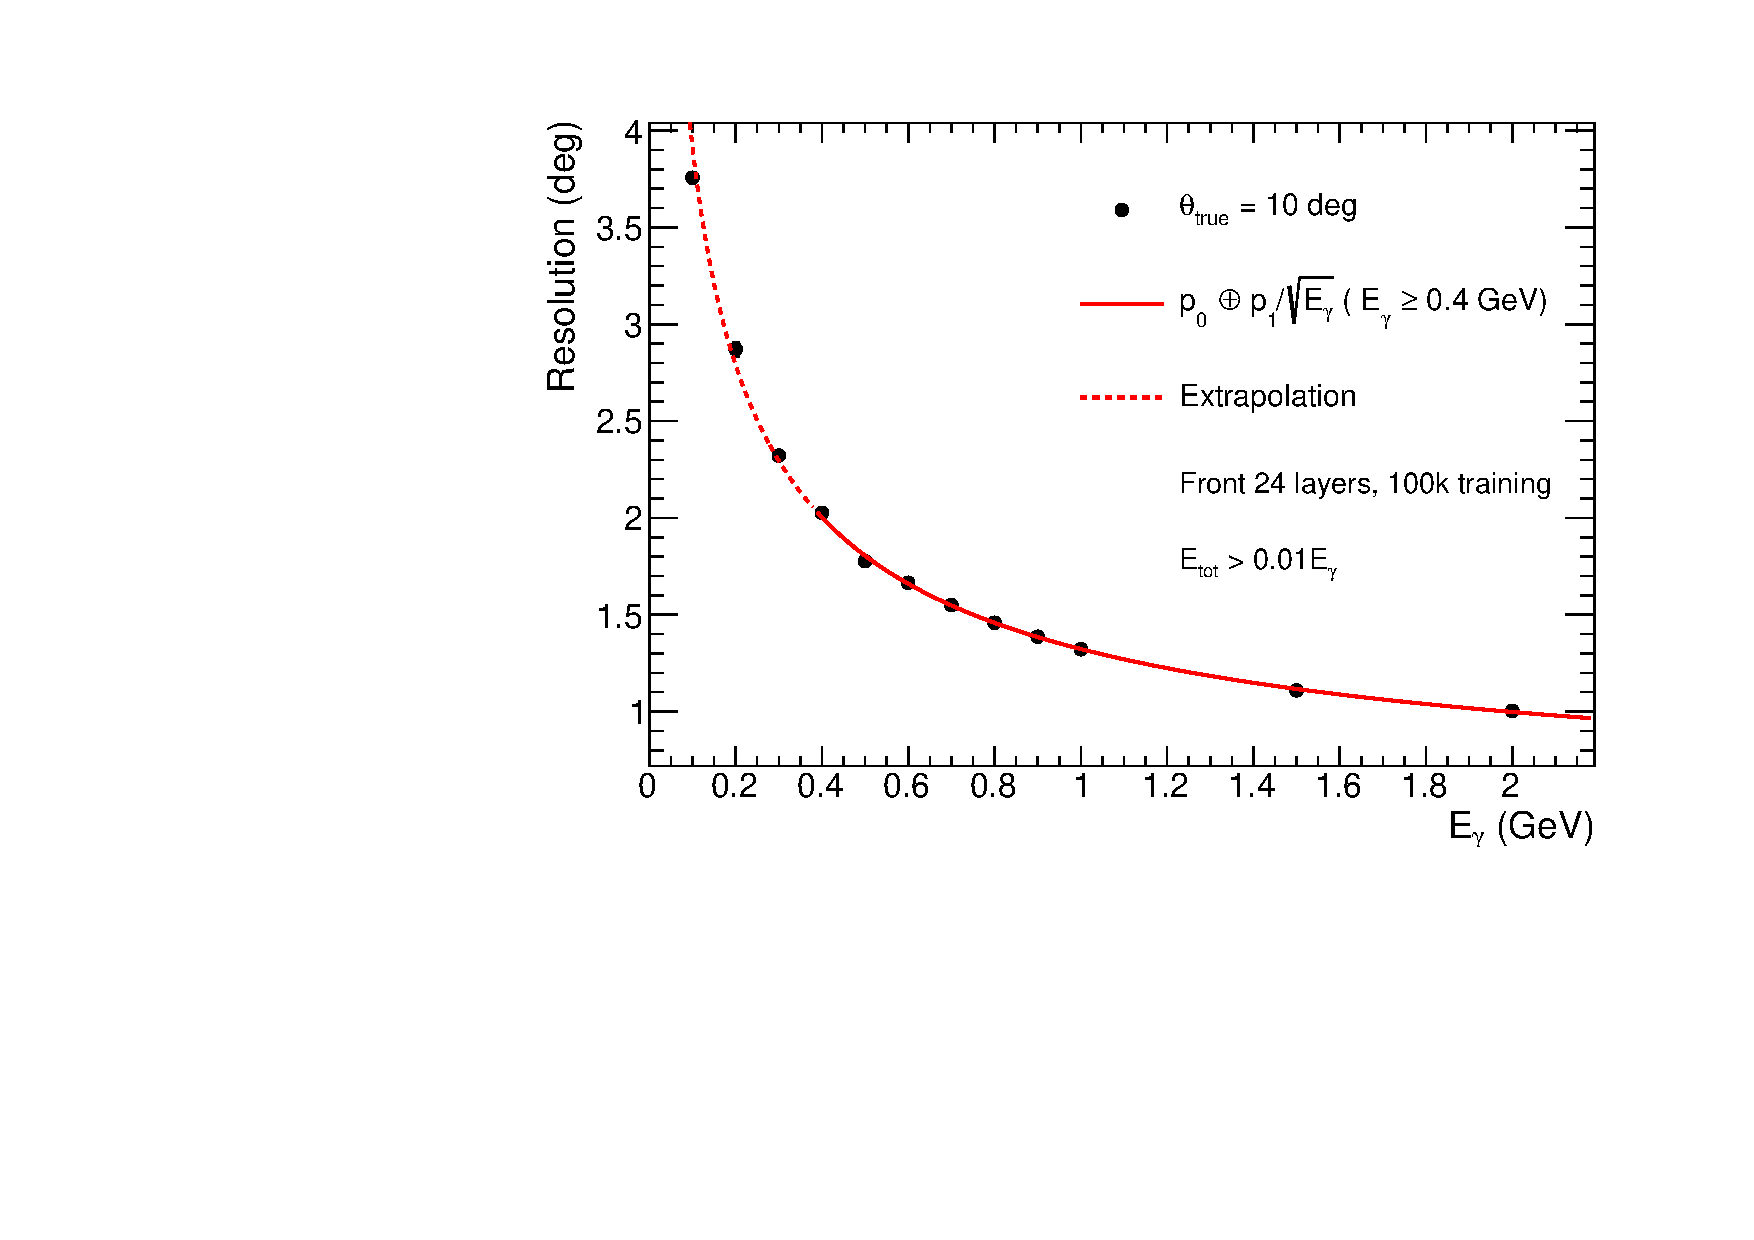
\includegraphics[width=0.5\textwidth]{figures/Fig7_Fit_eres.pdf}
}
\caption{ Angular resolutions as functions of the incidence angle for different incident energies (a) and the incident energy for $\theta=$~25$^{\circ}$, which is fitted with $p_{0} \oplus p_{1}/\sqrt{E_{\gamma}(GeV)}$ (b) }
\label{fig:angle_reco_dep_gr}
\end{figure}

Figure~\ref{fig:angle_reco_dep_gr} (a) shows the angular resolution as a function of the incidence angle for different incident energies ($E_{\gamma}$). The angular resolution does not depend on the incidence angle for high incident energy. On the other hand, the angular resolution is especially changing for low incident energy at the small incidence angle. Figure~\ref{fig:angle_reco_dep_gr} (b) shows the angular resolution as a function of the incident photon energy at $\theta=$~25$^{\circ}$. Angular resolutions are fitted with a function of $p_{0} \oplus p_{1}/\sqrt{E_{\gamma}(GeV)}$, where $p_{0}$ and $p_{1}$ represent an energy independent and energy dependent contribution, respectively.

\begin{figure}[!hbt]
\centering
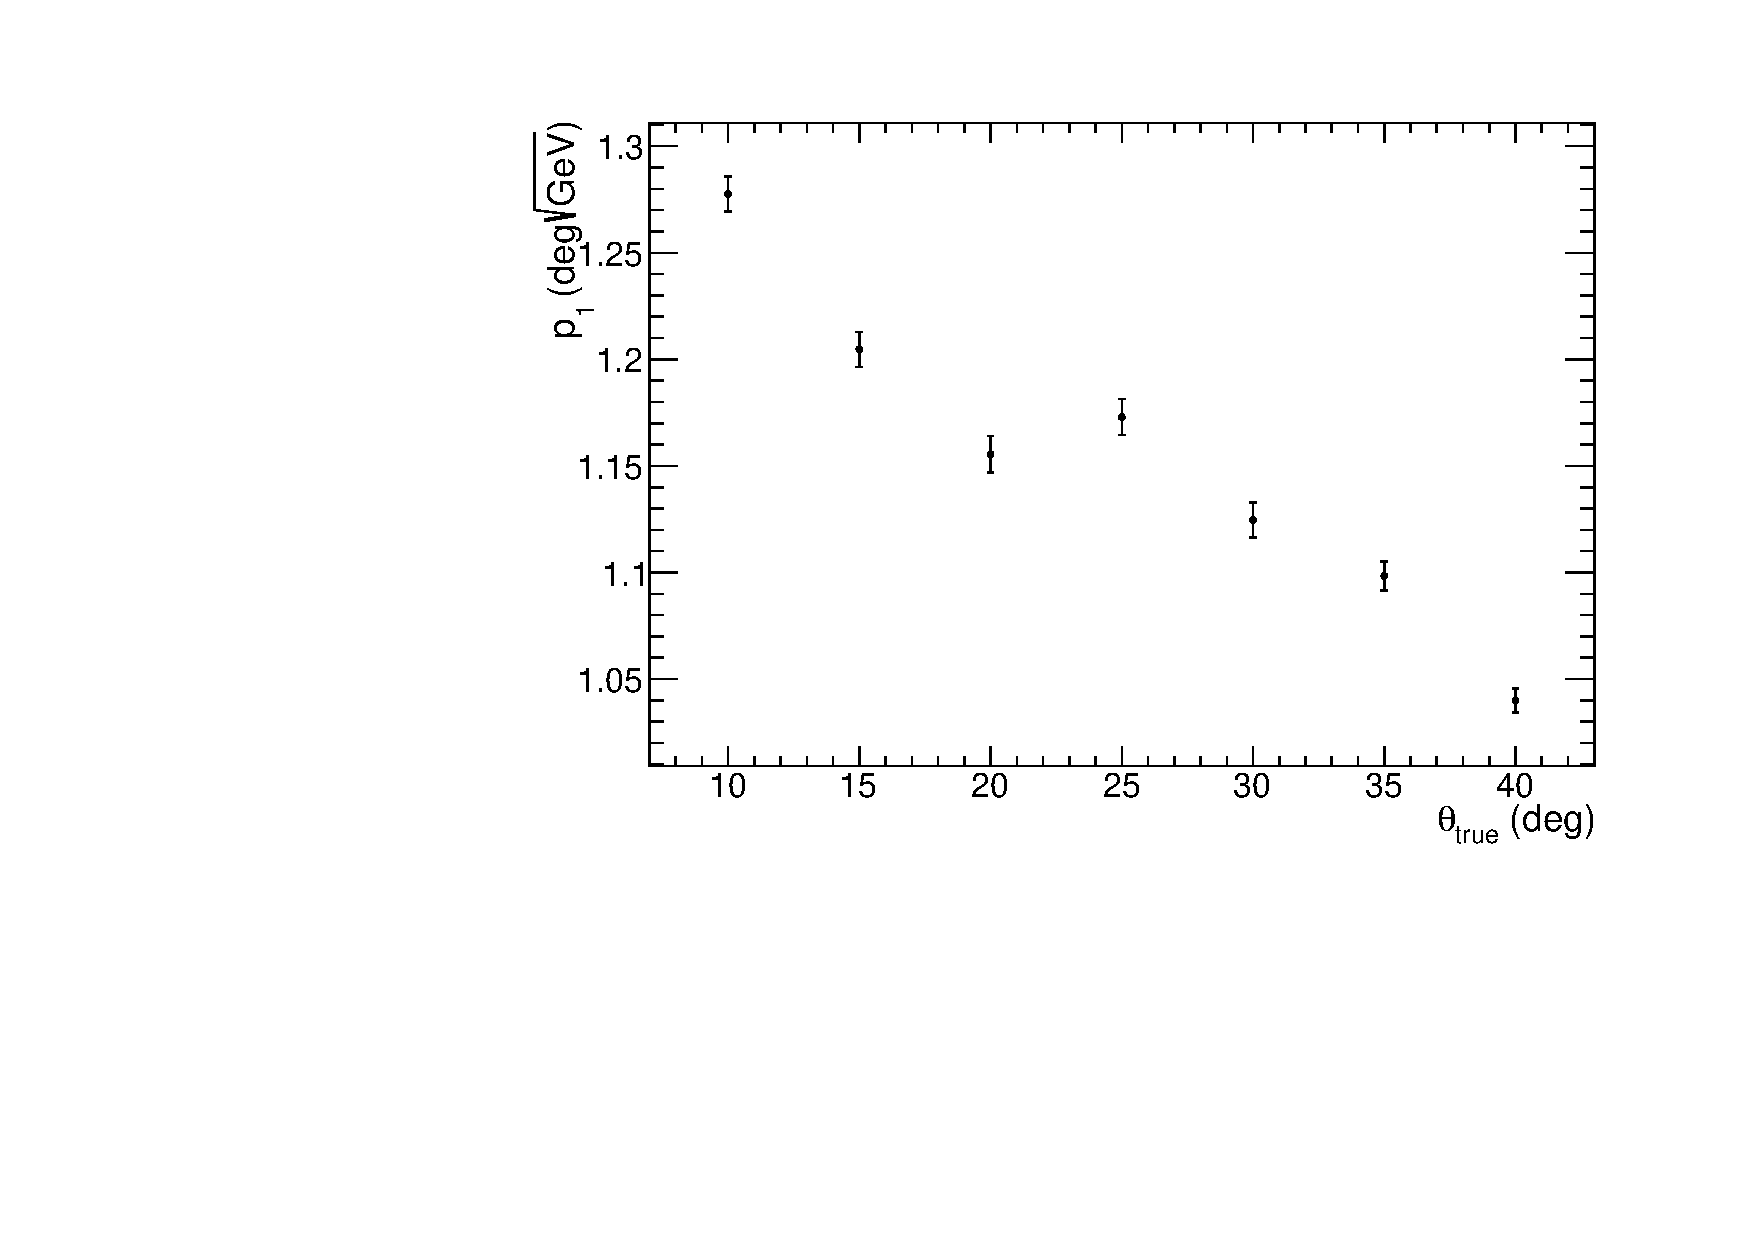
\includegraphics[width=0.58\textwidth]{figures/Fig7_eres_40deg.pdf}
\caption{ $p_{1}$ as a function of the incidence angle }
\label{fig:res_edep}
\end{figure}

Figure~\ref{fig:res_edep} shows estimated $p_{1}$ as a function of the incidence angle. $p_{0}$ and $p_{1}$ are consistent for $\theta>$~10$^{\circ}$ and estimated to be 0.29$^{\circ}$ and 1.24$^{\circ}$, respectively. For small $\theta$, $p_{1}$ is smaller than larger $\theta$ as the angular resolution is significantly dependent on the incidence angle for the low incident energy.

\begin{figure}[!hbt]
\centering
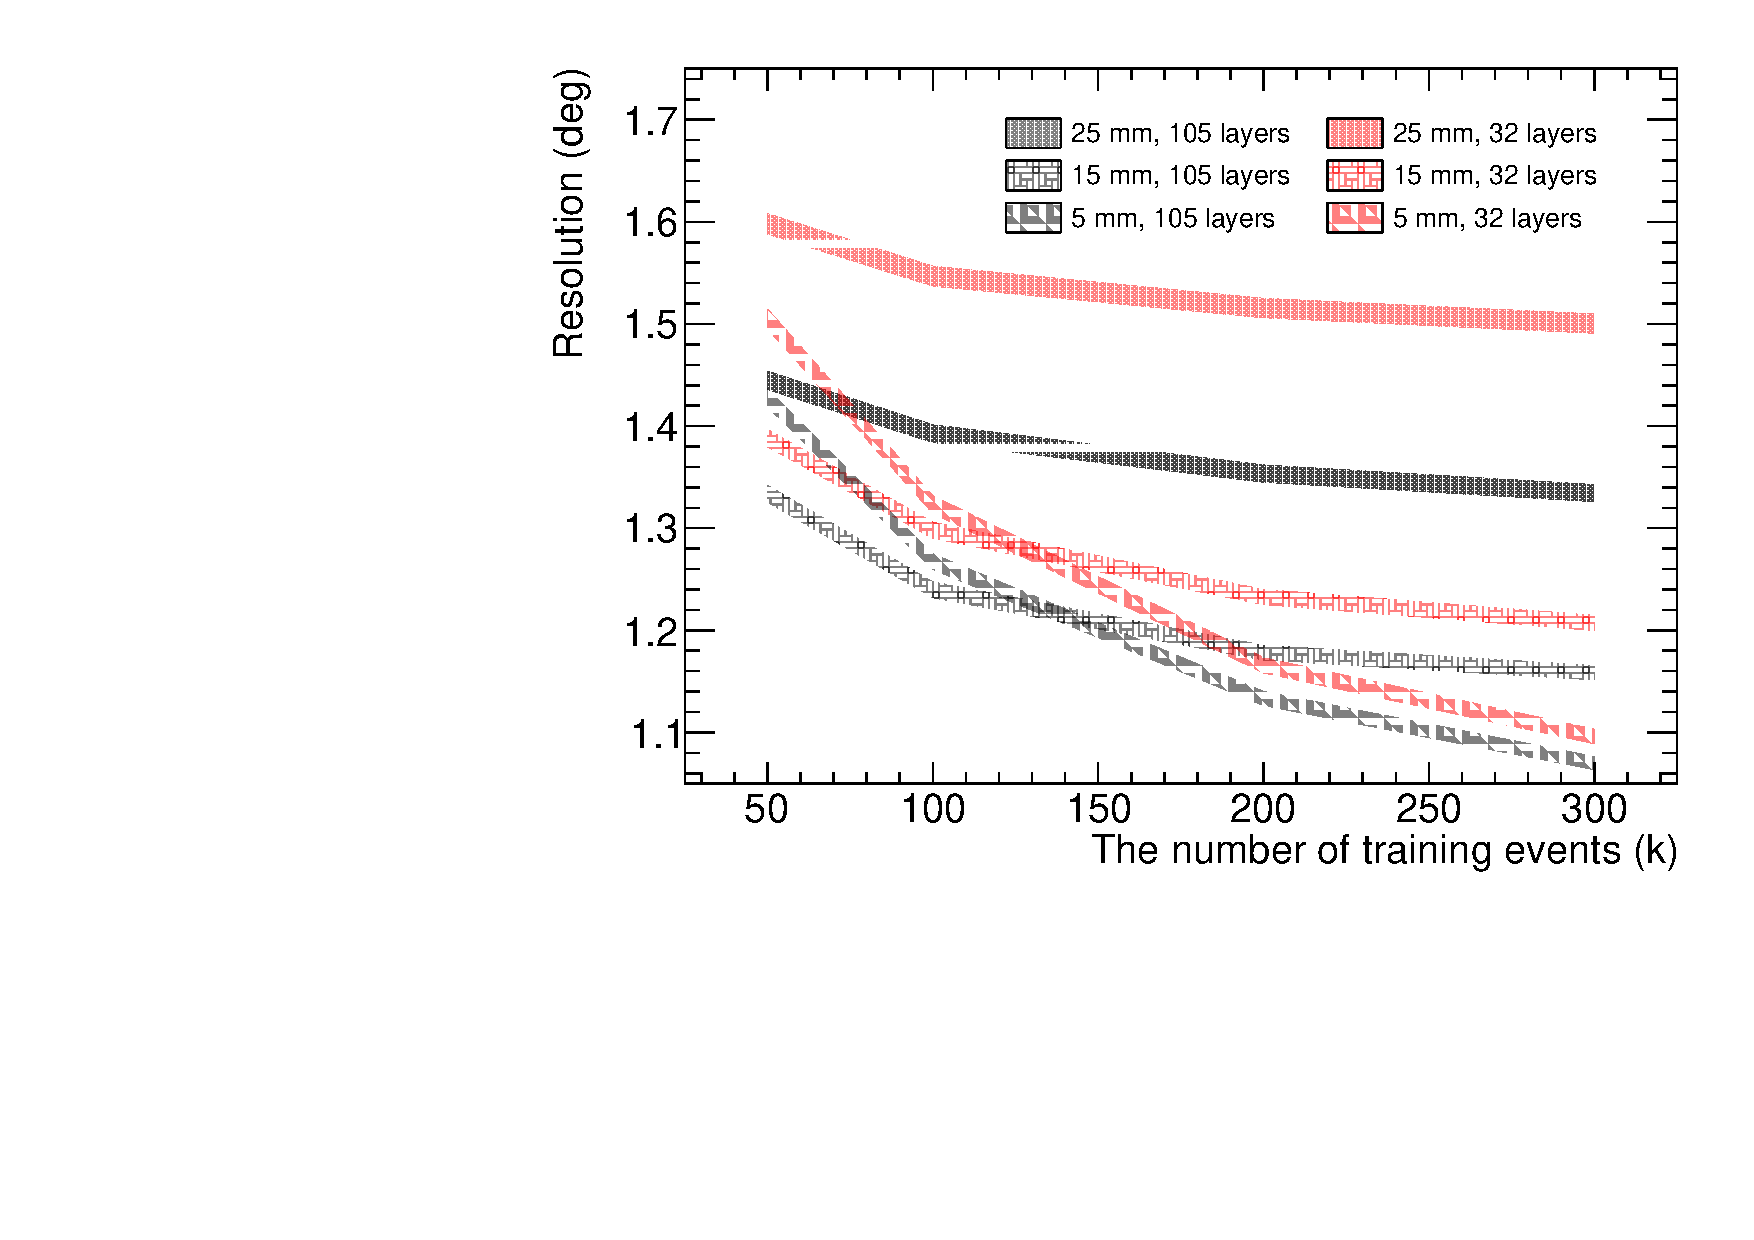
\includegraphics[width=0.6\textwidth]{figures/Fig8_nsample.pdf}
\caption{ The angular resolution for 1-GeV photons at $\theta=$~10$^{\circ}$ as a function of the number of training samples with different strip widths using the first 24 layers or the full layers. }
\label{fig:multi-parameter}
\end{figure}

Figure~\ref{fig:multi-parameter} shows the angular resolution with different numbers of training samples for different detector configurations. All configurations show a decrease in the angular resolution with increasing training samples, which means that enhanced statistics for the training results in better reconstruction. The angular resolution with 5-mm-wide scintillator strips decreases more rapidly than others. The number of features for the 5-mm-wide strip is much larger than others, and the number of training samples is much required to correlate larger features. Considering limited computing resources, the setup with $10^{5}$ events, 24 layers, and the 15-mm-wide strip was chosen for training the XGB model. The training result differs by only 0.2$^{\circ}$ from the best setup will full layers.
 
\section{SUMMARY}
\label{sec:sum}

We report simulation results on the incidece angle reconstruction of EM sampling calorimeters with photons being in the range of 100~MeV to 2~GeV. EM shwers are simulated in the new samplinng calorimeter.using Geant4. We utilize the XGB model to reconstruct the photon incident angle by correlating all energy deposits in each strip with the incidence angle all events together.

We tune the hyperparameter of the XGB to reconstruct the incidence angle with the best angular resolution, and study the angular resolution in terms of the detector configuration. We find that 15-mm-wide strips provide the best angular resolution of 1.23~$\pm$~0.01$^{\circ}$. We also conclude that using 24 front layers gives the acceptable angular resolution of 1.33~$\pm$~0.01$^{\circ}$, which is only 0.1$^{\circ}$ higher than the angular resolution we get from the full layer. We evaluate angular resolutions in terms of the incidence angle and the incident energy. The angular resolution can be expressed as $p_{0} \oplus p_{1}/\sqrt{E_{\gamma}(GeV)}$. $p_{0}$ is estimated to be 0.43$^{\circ}$ and not dependent on the incidence angle. $p_{1}$ is estimated to be 1.28--1.04$^{\circ}$ and gradually decreasing with the incidence angle.

Furthermore, we study that the angular resolution is changing with the variation of the training of the XGB and the detector configuration. As the strip width decreases, more channels of scintillator strips are required, and the training of the XGB gets affected due to the increased feature size. This is quenched with the larger number of training samples, which qualitatively improves the training of the XGB. On the other hand, the longer strip width provides the worse angular resolution as the position resolution of the EM shower gets worse. We conclude that 15-mm-wide strips provide the favorable angular resolution with 24 front layers and $10^{5}$ training samples.

\label{sec:con}

%\pagebreak

\section*{Acknowledgement}
This paper was supported by the National Research Foundation of Korea (NRF) grants funded by the Korea government (MIST) (2019R1A2C1084552 and \\ 2020R1A3B2079993).

\printbibliography

\end{document}
